\clearpage
\chapter{B Parking Trigger Strategy}\label{sec:triggers}

The analysis' signal process contains displaced SM $\tau$ leptons in its final state. 
In order to exploit the leptonic decay of $\tau$ lepton with significant IP, specifically with muon final state for clean signal, the B-Parking triggers are used. 
CMS implemented the B-Parking trigger since the year of 2018 of Run 2 for research on lepton universalities. 
For research of R(K$^{*}$,D$^{*}$), muonic final state of B mesons are desired. 
B trigger requires a soft muon with modest displacement (measured using impact parameter) from the primary vertex, exploiting the b quark's long lifetime.
B Parking trigger requires a muon with transverse momentum (pT) of 7-12 GeV with impact parameter (IP) 3-6.
pp collisions in LHC produce extremely enormous amount of events, which could trigger the B parking trigger paths. 
Current CPU capacity of CMS is limited and not capable of reconstructing the entire event at such high trigger rate in HLT level.
Thus, CMS scouts events, meaning it writes events that passed L1 trigger to a temporary dataset. Later, full HLT and RECO steps are implemented and served as a B-Parking dataset. 
The prescale factor for BPH triggers is 5-6.
\begin{figure}[h!]
  \caption{eeeddd}
  \label{fig:Lepton}
  \centering
  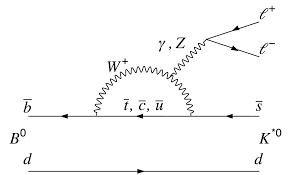
\includegraphics[width=0.57\linewidth]{figs/LU1.png}
  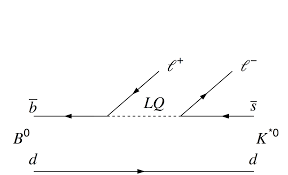
\includegraphics[width=0.57\linewidth]{figs/LU2.png}

\end{figure}


\section{Global Tags}
\begin{table}[htb]
\caption{Data and MC Global tags used 2018}
\begin{center}
\begin{tabular}{r|l}\hline
 Data 2018 & 106X\_dataRun2\_v29 \\
 \hline
 MC 2018   & 106X\_upgrade2018\_realistic\_v11\_L1v1 \\
 \hline
\end{tabular}
\label{tab:GT}
\end{center}
\end{table}


\section{Trigger Paths}
We utilize the B-Parking triggers collecting data for the year of 2018.
The exact names of paths for B-Parking triggers are listed in Table~\ref{tab:triggers18}.
We observe that the trigger efficeincy reaches a plateau after requiring a muon with pT value above that utilizes in the L1 seed.
%The standard trigger scale factors are applied in order to correct the MC.

\begin{table}[htb]
\caption{HLT trigger paths used in the analysis 2018.}
\begin{center}
\begin{tabular}{r|l}\hline
\hline
 Data sample & Trigger \\
\hline
 ParkingBPH*-Run2018A & HLT\_Mu9\_IP6\_part* \\
 \hline
 ParkingBPH*-Run2018B & HLT\_Mu12\_IP6\_part* \\
 ParkingBPH*-Run2018C & HLT\_Mu12\_IP6\_part* \\
 ParkingBPH*-Run2018D & HLT\_Mu12\_IP6\_part* \\
 \hline
 \hline
\end{tabular}
\label{tab:triggers18}
\end{center}
\end{table}

Below is the trigger efficiency of various BPH trigger paths for different mass and lifetime points of the signal (HToSSTo4Tau) sample
\begin{figure}[h!]
  \caption{asd}
  \label{fig:Trigger Efficiency}
  \centering
  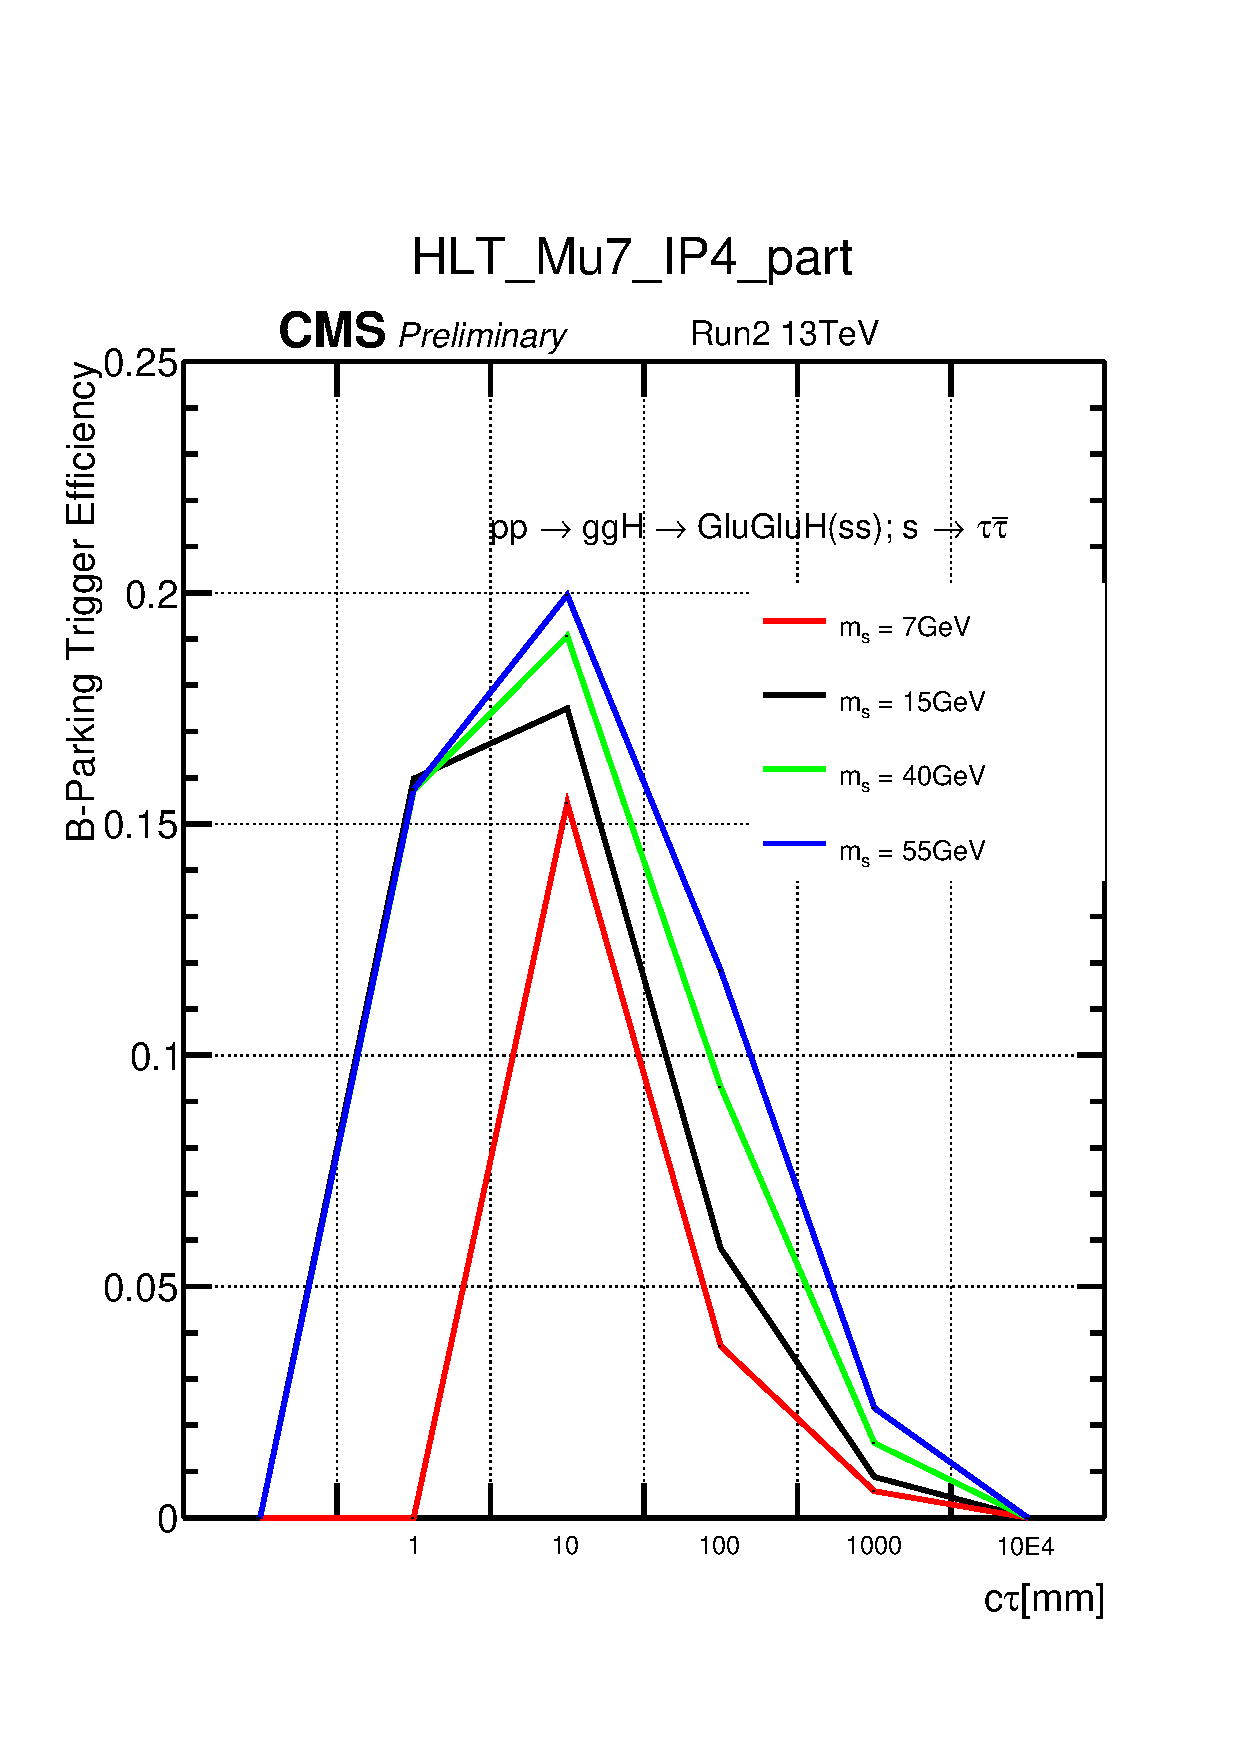
\includegraphics[width=0.47\linewidth]{figs/TrigEff_HLT_Mu7_IP4_part.pdf}
  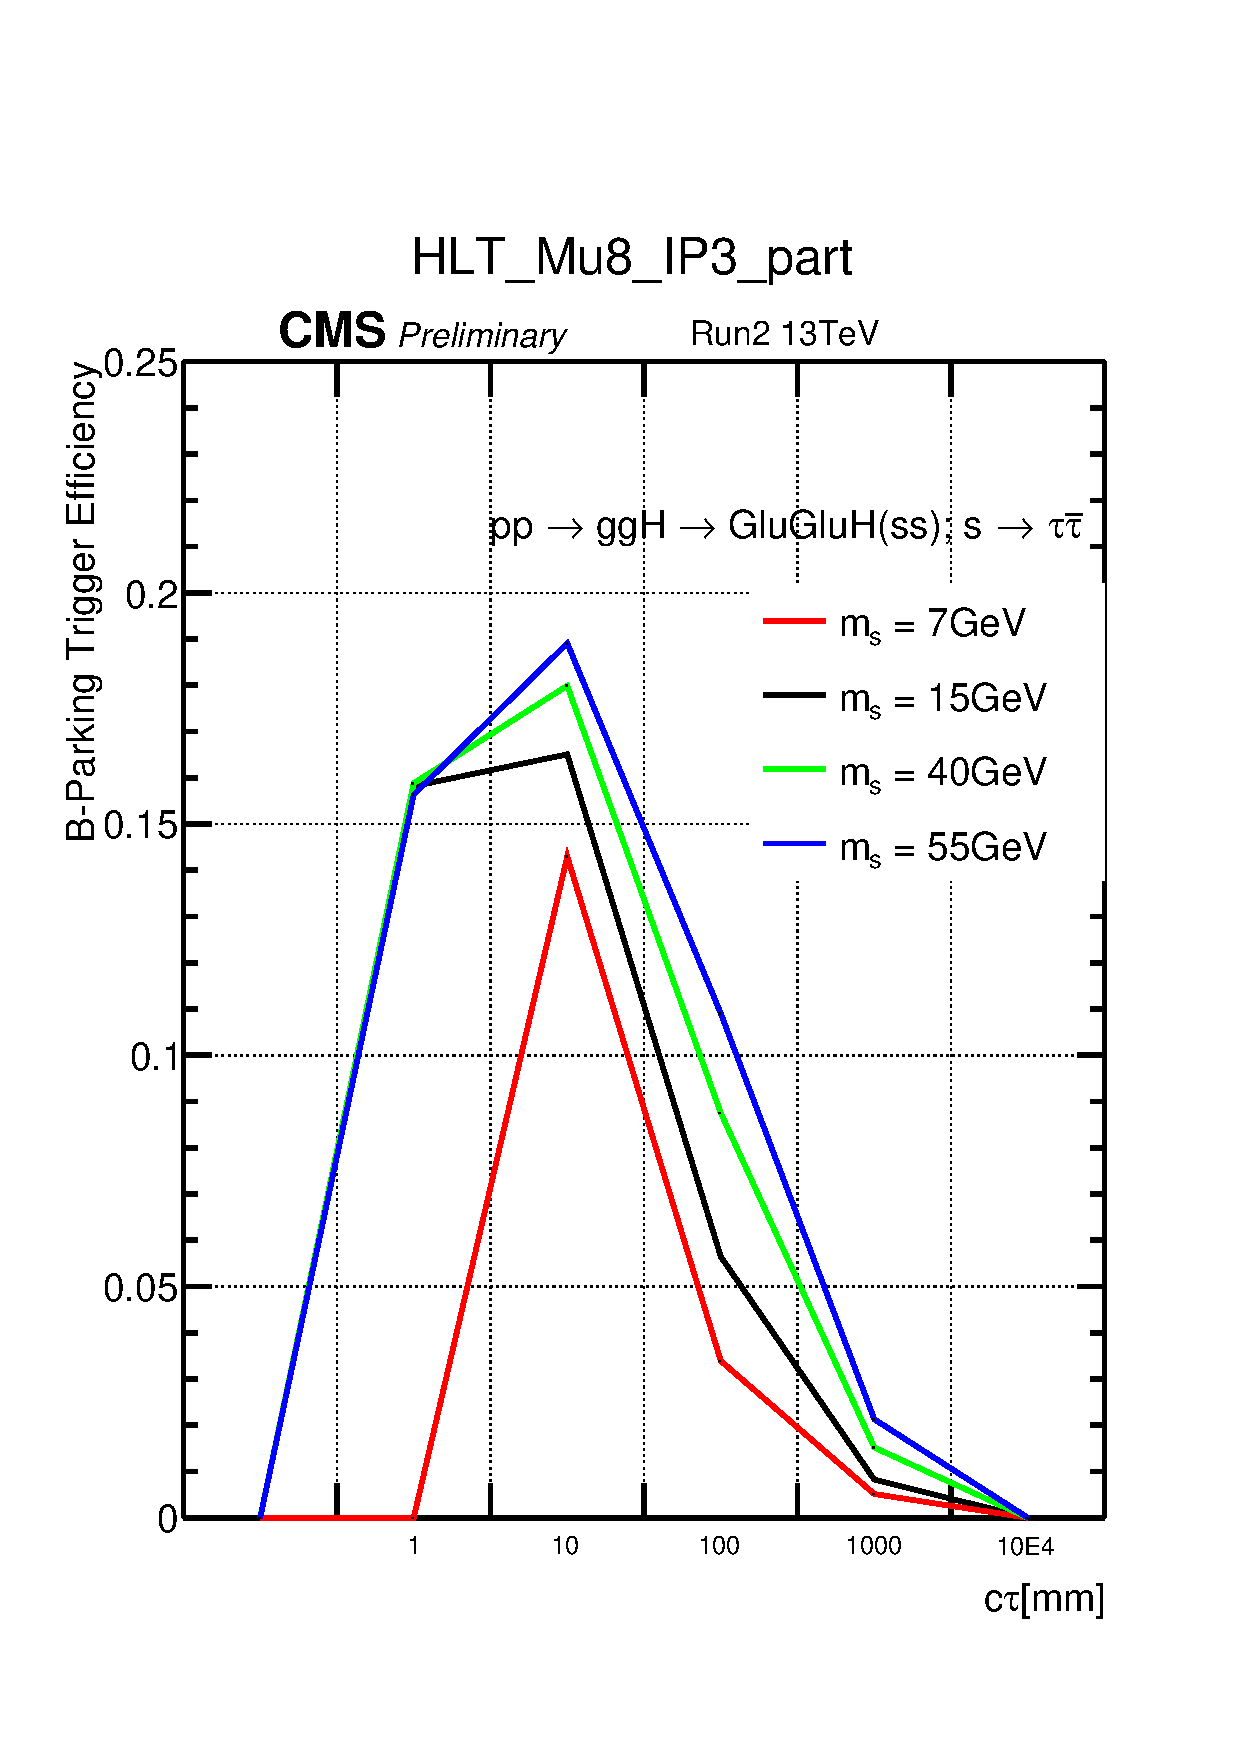
\includegraphics[width=0.47\linewidth]{figs/TrigEff_HLT_Mu8_IP3_part.pdf}

\end{figure}
\begin{figure}[h!]
  \caption{eeee}
  \label{fig:Trigger Efficiency2}
  \centering
  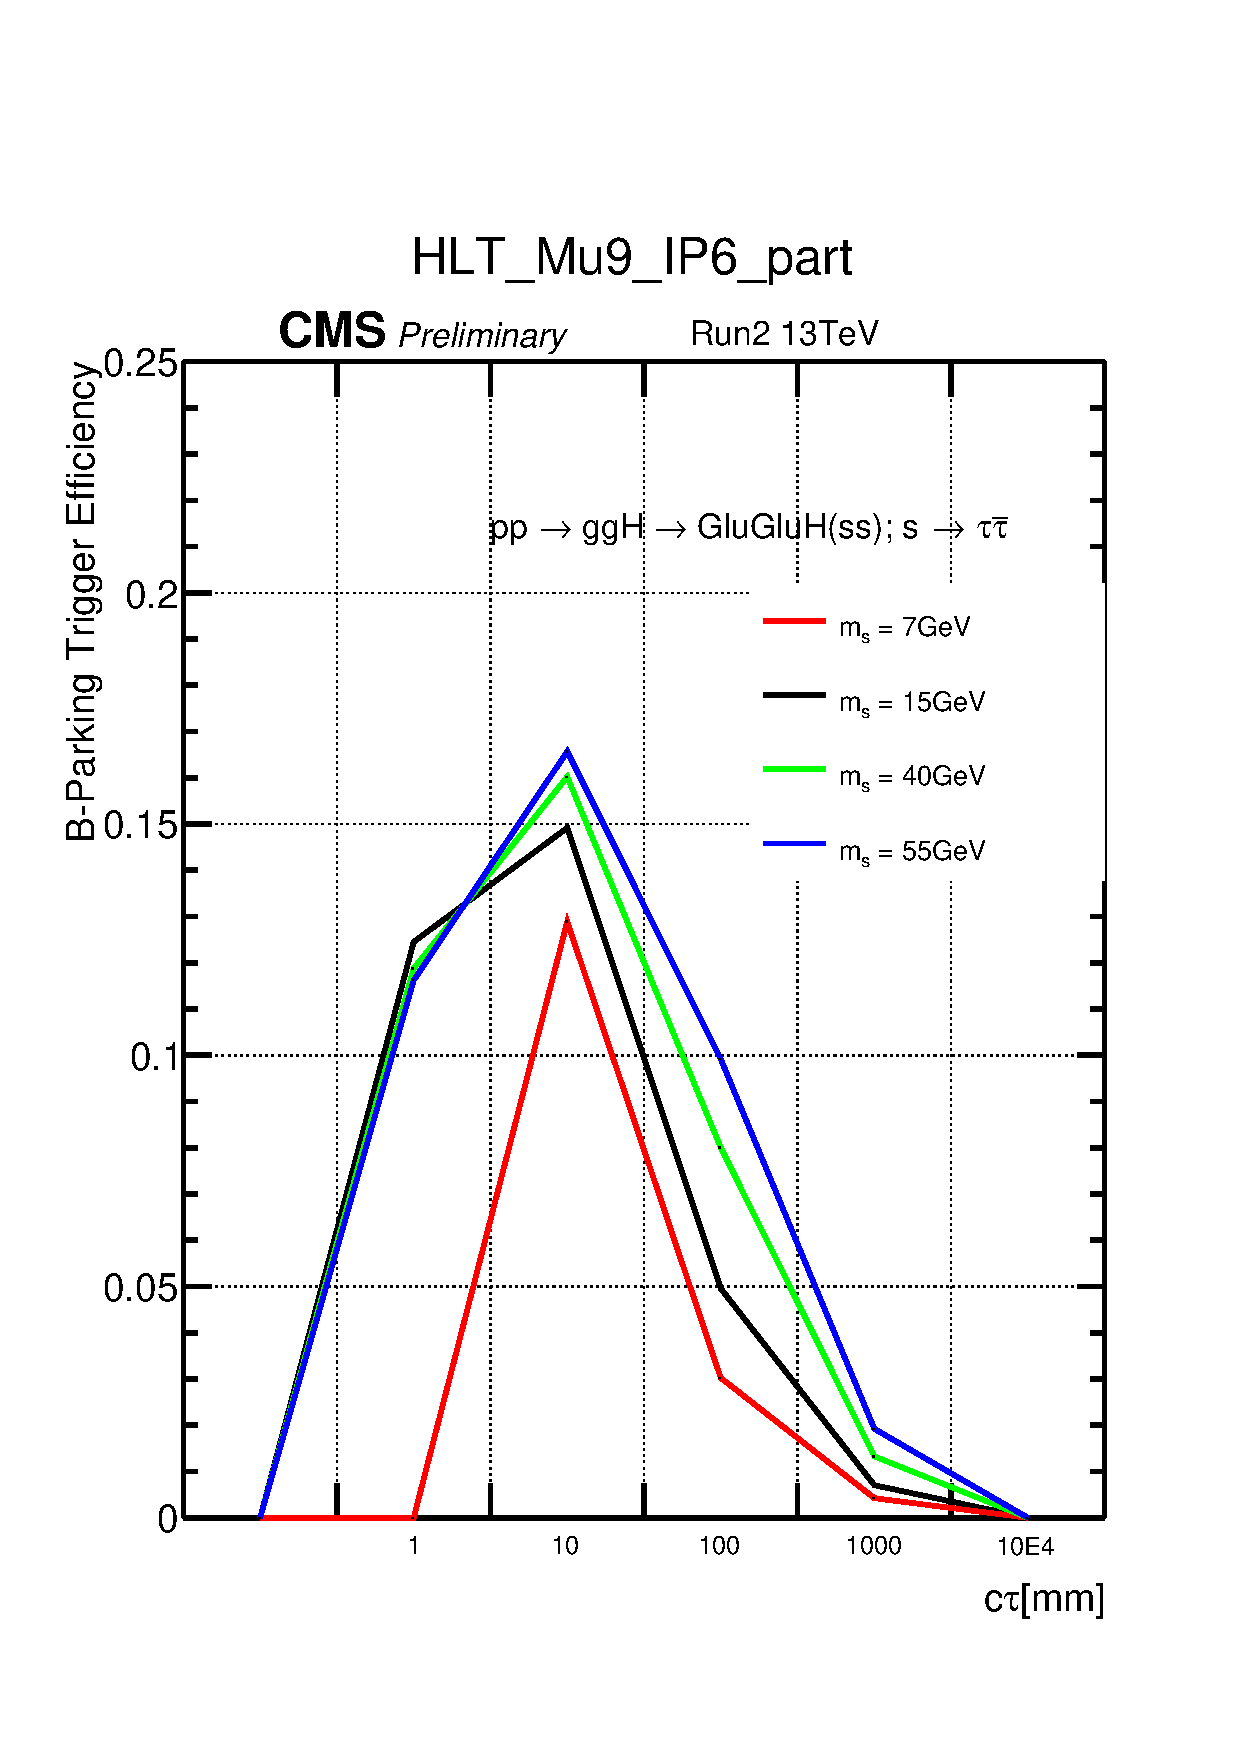
\includegraphics[width=0.47\linewidth]{figs/TrigEff_HLT_Mu9_IP6_part.pdf}
  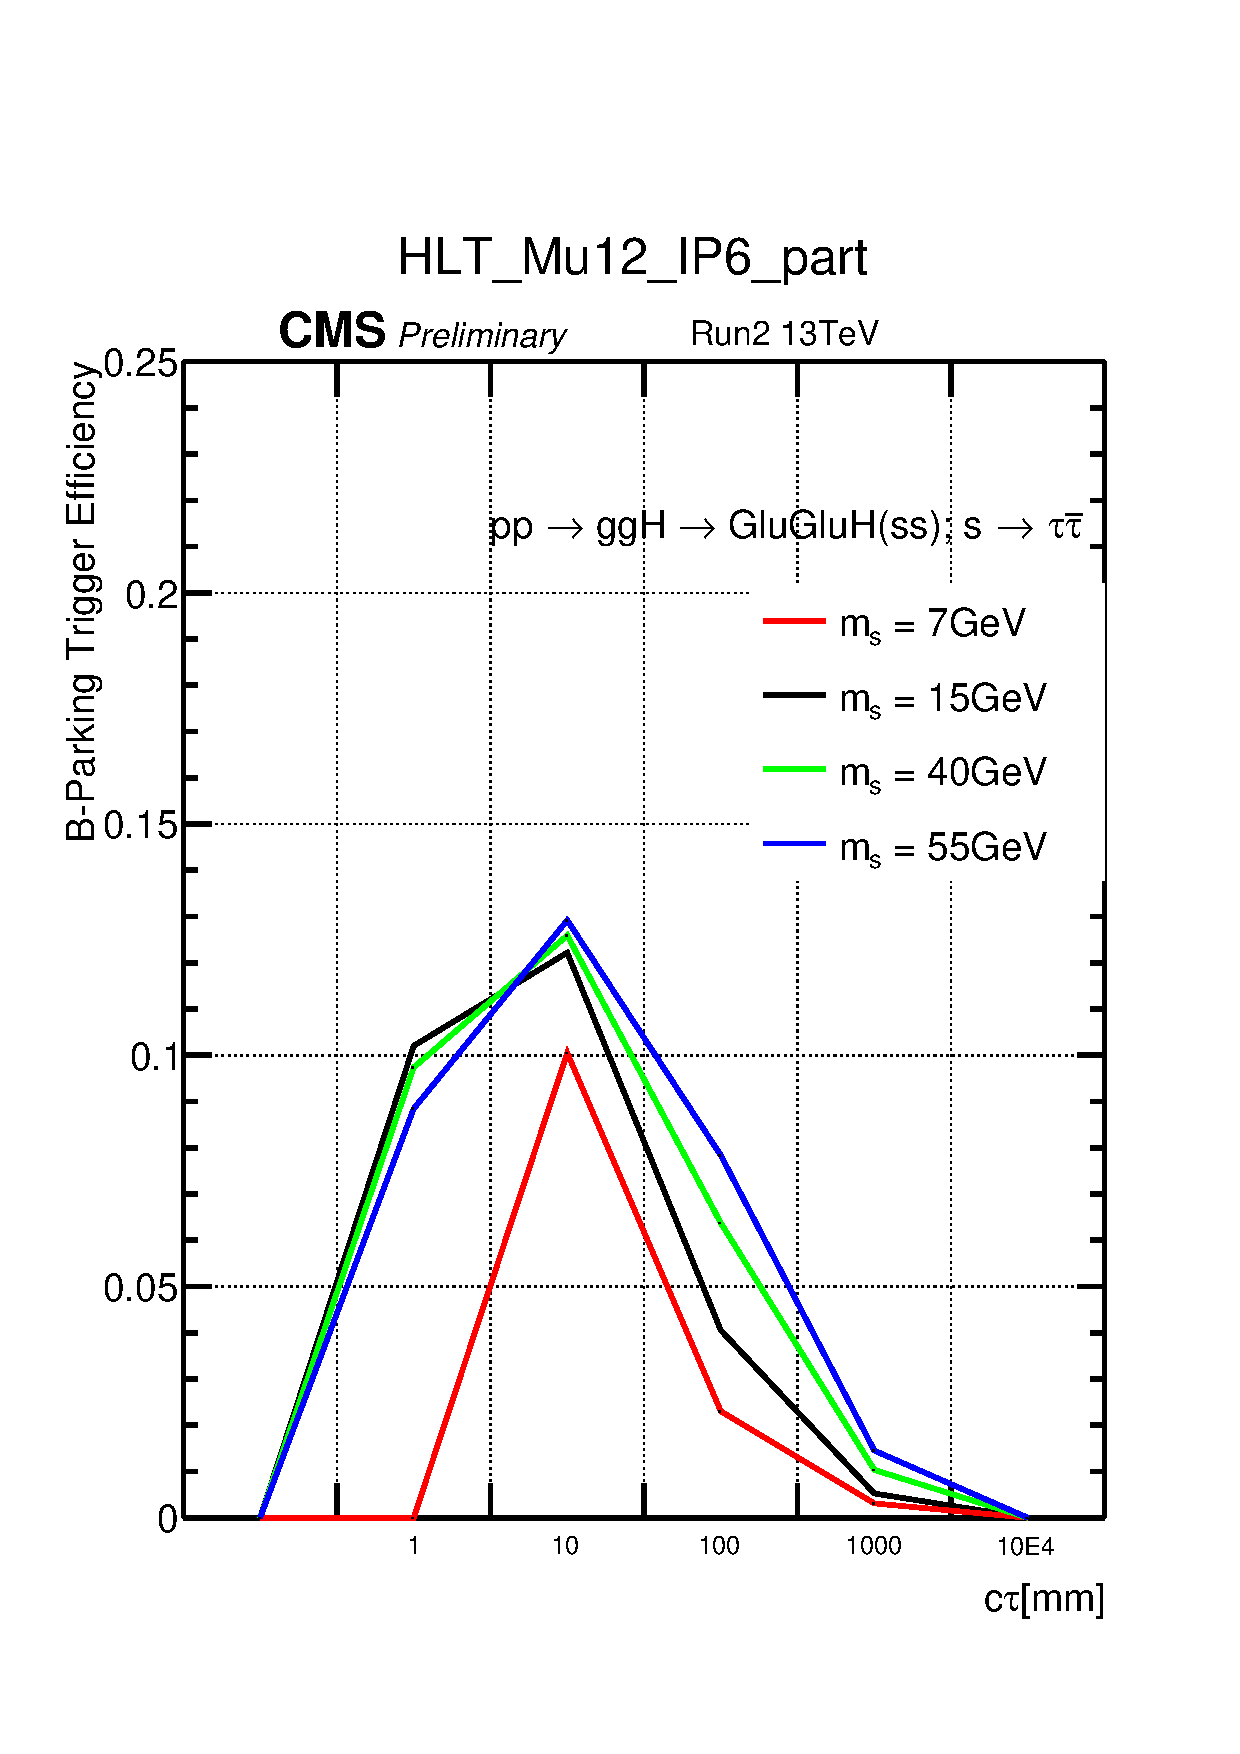
\includegraphics[width=0.47\linewidth]{figs/TrigEff_HLT_Mu12_IP6_part.pdf}

\end{figure}
